\documentclass[
  11pt,
  letterpaper,
   addpoints,
  answers
  ]{exam}

% Carga el preámbulo localizado en la carpeta superior
\NeedsTeXFormat{LaTeX2e}[2023/04/30]

% Provide the name of your page, the date it was last updated, and a comment about what it's used for
\ProvidesPackage{../exercise-preamble}[2023/04/30 Prof. Cassanelli custom LaTeX style]

% \usepackage{printlen}
% \uselengthunit{in}\printlength{\textwidth}

% PACKAGES
\usepackage[dvipsnames]{xcolor}

\usepackage{graphicx}
\graphicspath{{../figures}}
\usepackage{amsmath,amsthm,amssymb,mathtools,mathrsfs}
\usepackage{commath}
\usepackage{upgreek}
\usepackage{cancel}
\usepackage{enumerate}
\usepackage[font=small]{caption}
\usepackage[normalem]{ulem}
\usepackage{steinmetz}

\usepackage[left=1.5cm, right=1.5cm, top=1cm]{geometry}

% REFERENCES AND OTHERS
\usepackage{../aas_macros}
\usepackage{natbib}
\bibpunct{(}{)}{;}{a}{}{,}

\usepackage{tikz}
\usepackage{tikz-3dplot}
\usepackage{circuitikz}
\usepackage{pgfplots}
\pgfplotsset{compat=1.15}
\usepgfplotslibrary{smithchart}
\usetikzlibrary{
  decorations.pathmorphing,
  decorations.markings,
  calc,
  patterns,
  decorations,
  angles,
  quotes,
  ext.topaths.arcthrough,
  shapes
  }

\usepackage{siunitx}
\sisetup{
    range-phrase=\text{--},
    range-units=single,
    separate-uncertainty=true,
    print-unity-mantissa=false
    }
\DeclareSIUnit{\gauss}{G}
\DeclareSIUnit{\jansky}{Jy}

\newcommand{\iu}{\mathrm{i}\mkern1mu}
\newcommand{\ju}{\mathrm{j}\mkern1mu}
\newcommand{\euler}{\mathrm{e}}
\newcommand{\exponential}[1]{\mathrm{exp}\left[#1\right]}
\newcommand{\uvec}[1]{\widehat{\mathbf{#1}}}
\newcommand{\uvecs}[1]{\boldsymbol{\widehat{#1}}}
\newcommand{\bvec}[1]{\boldsymbol{\mathcal{#1}}}

\usepackage{hyperref}
\hypersetup{
    % bookmarks=true,
    unicode=true,
    pdftoolbar=true,
    pdfmenubar=true,
    pdffitwindow=false,
    pdfstartview={FitH},
    pdftitle={EL3103},
    pdfauthor={Tomas Cassanelli},
    pdfcreator={Tomas Cassanelli},
    pdfnewwindow=true,
    colorlinks=true,
    linkcolor=Violet,
    citecolor=Violet,
    urlcolor=Violet
    }

% Exam document class
\renewcommand{\figurename}{Figura}
\renewcommand{\tablename}{Cuadro}
\pagestyle{empty}

\usepackage[spanish]{cleveref}

\crefname{question}{\protect{pregunta}}{\protect{preguntas}}
\Crefname{question}{\protect{Pregunta}}{\protect{Preguntas}}
\creflabelformat{question}{#2{#1}#3}

\renewcommand{\solutiontitle}{\noindent\textbf{Solución:}\par\noindent}
\bracketedpoints
\pointname{~puntos}

\endinput

% Paquetes locales
\usepackage{float}
\usepackage{booktabs} % para \toprule, \midrule, \bottomrule
\usepackage{xcolor} % para colores
\usepackage{bm} % para negrita en símbolos matemáticos

% Macros locales
\newcommand{\Rel}{\mathfrak{R}} % símbolo para la reluctancia

\begin{document}

% Configuración del encabezado usando comandos de la clase exam
\pagestyle{headandfoot}
\extraheadheight{0.5in} % Baja el encabezado aumentando el espacio superior
\firstpageheader{\textit{Análisis de Sistemas Dinámicos y Estimación}}{}{EL3204-1}
\runningheader{\textit{Análisis de Sistemas Dinámicos y Estimación}}{}{EL3204}
\firstpagefooter{}{\thepage}{}
\runningfooter{}{\thepage}{}
\headrule % Línea debajo del encabezado

% Numeración de página
\pagenumbering{arabic}

% Portada
\begin{center}
    \vspace*{1cm}
    
    % Logo superior
    \includegraphics[width=0.5\textwidth]{../fcfm_die}
    
    \vspace{2cm}
    
    % Líneas decorativas superiores
    
\begin{tikzpicture}
        \draw[line width=2pt, black!70] (0,0) -- (10,0);
        \draw[line width=0.5pt, black!50] (0,0.2) -- (10,0.2);
    \end{tikzpicture}
    
    \vspace{1cm}
    
    % Título principal
    {\fontsize{28}{34}\selectfont\bfseries 
    Análisis de Sistemas\\[0.3cm]
    Dinámicos y Estimación}
    
    \vspace{0.5cm}
    
    {\Large\textbf{EL3204-1}}
    
    \vspace{1cm}
    
    % Líneas decorativas inferiores
    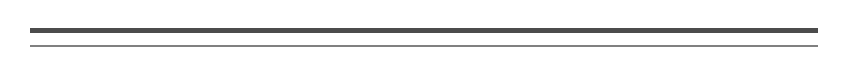
\begin{tikzpicture}
        \draw[line width=0.5pt, black!50] (0,0) -- (10,0);
        \draw[line width=2pt, black!70] (0,0.2) -- (10,0.2);
    \end{tikzpicture}
    
    \vspace{1.5cm}
    
    % Subtítulo
    {\LARGE\itshape Pauta Auxiliar 10 - Auxiliar Extra C2}
    
    \vspace{0.5cm}
    {\large Prof Marcos Orchard - Sebastian Espinoza.}\\
    {\large Prof Auxiliar Erik Sáez Aravena.}
    
    % Decoración con símbolo matemático de fondo
    \begin{tikzpicture}[remember picture, overlay]
        \node[opacity=0.5, rotate=0] at ([yshift=-8cm]current page.center) {
            \fontsize{200}{220}\selectfont\color{black!15}$\mathbb{E}[\Theta|X]$
        };
    \end{tikzpicture}
    
    \vfill
    
\end{center}

\newpage
%----------------------------
% =========================================
% Unidad II — Detección Bayesiana (Resumen)
% =========================================
\section*{Resumen}

En esta unidad se presenta la perspectiva bayesiana: en lugar de asumir un parámetro desconocido fijo se modela \(\Theta\) como una variable aleatoria con una distribución a priori que refleja la creencia del agente. Las observaciones actualizan esa creencia mediante la regla de Bayes y, dado un esquema de costos, la decisión óptima minimiza el riesgo posterior. Desde un enfoque subjetivista la prior no tiene que describir un mecanismo físico, sino que recoge información previa del detector; esto permite un tratamiento más flexible de la incertidumbre en problemas de detección y estimación.

En el contexto Bayesiano, \(\Theta\) se modela como una variable aleatoria con valores en \(\mathcal{A} = \{1,\ldots,k\}\) y distribución a priori \(p_\Theta(\theta)\). Dada una observación \(X\), la probabilidad condicional se expresa mediante la regla de probabilidad condicional:
\[
\mathbb{P}(X(w) \in B|\Theta(w) = \theta) = P_{X|\Theta}(B,\{\theta\}) = P_\Theta(\{\theta\}) \cdot P_{X|\Theta}(B|\{\theta\}).
\]
Para un vector conjunto \((X,\Theta)\), la distribución conjunta queda determinada por:
\[
\mathbb{P}(X(w) \in B, \Theta(w) = \theta) = P_{X,\Theta}(B,\{\theta\}) = p_\Theta(\theta) \cdot \int_B f_{X|\Theta}(x|\theta)\,dx
\]
en el caso continuo, o bien
\[
\mathbb{P}(X(w) \in B, \Theta(w) = \theta) = P_{X,\Theta}(B,\{\theta\}) = p_\Theta(\theta) \cdot \sum_{x \in B} p_{X|\Theta}(x|\theta)
\]
en el caso discreto. Con esto, un problema de detección Bayesiano consiste en definir un espacio de observación \(\mathbb{X}\), un espacio de decisión \(\mathcal{A}\), las distribuciones condicionales \(P_{X|\Theta}(\cdot|\theta)\) o densidades \(f_{X|\Theta}(\cdot|\theta)\), una regla de decisión (test) \(\pi: \mathbb{X} \to \mathcal{A}\) y una función de costo \(L: \mathcal{A} \times \mathcal{A} \to \mathbb{R}^+ \cup \{0\}\) que penaliza decisiones incorrectas.
\begin{itemize}
\item \textbf{Riesgo Promedio Bayesiano:} Para encontrar la regla óptima, se busca minimizar el riesgo promedio Bayesiano, que es el promedio del costo dado por \(L(\Theta, \pi(X))\). Primero se define el \emph{riesgo promedio} condicionado a \(\Theta = \theta\):
\[
R(\theta, \pi) \triangleq \mathbb{E}(L(\theta, \pi(X))|\Theta = \theta) = 
\begin{cases}
\displaystyle\int_{\mathbb{X}} L(\theta, \pi(x)) f_{X|\Theta}(x|\theta)\,dx & \text{(caso continuo)} \\[0.5em]
\displaystyle\sum_{x \in \mathbb{X}} L(\theta, \pi(x)) p_{X|\Theta}(x|\theta) & \text{(caso discreto)}
\end{cases}
\]
El \emph{Riesgo Promedio Bayesiano} se obtiene promediando \(R(\theta, \pi)\) respecto a la distribución a priori de \(\Theta\):
\[
r(\pi) \triangleq \mathbb{E}_{\Theta}(R(\Theta, \pi)) = \sum_{\theta \in \mathcal{A}} R(\theta, \pi) \cdot p_{\Theta}(\theta) = \mathbb{E}_{X,\Theta}(L(\Theta, \pi(X))).
\]
La \emph{regla óptima Bayesiana} \(\pi^*\) es aquella que minimiza el riesgo promedio Bayesiano:
\[
\pi^* = \arg\min_{\pi \in F(\mathbb{X}, \mathcal{A})} r(\pi) = \arg\min_{\pi \in F(\mathbb{X}, \mathcal{A})} \mathbb{E}_{X,\Theta}(L(\Theta, \pi(X))).
\]
Equivalentemente, para cada observación \(x \in \mathbb{X}\), la decisión óptima \(\pi^*(x)\) minimiza el \emph{riesgo a posteriori}:
\[
\pi^*(x) = \arg\min_{y \in \mathcal{A}} \sum_{\theta \in \mathcal{A}} L(\theta, y) P_{\Theta|X}(\Theta = \theta|x) = \arg\min_{y \in \mathcal{A}} \mathbb{E}(L(\Theta, y)|X = x).
\]
\item \textbf{Función de costo 0-1 y regla MAP:} La función de costo 0-1 juega un rol fundamental en problemas de reconocimiento de patrones y comunicaciones digitales, pues su costo promedio equivale a la probabilidad de error de decisión. Se define como:
\[
L_{0,1}(x, y) = 
\begin{cases}
0 & \text{si } x = y \\
1 & \text{si } x \neq y
\end{cases}
\quad \forall x, y \in \mathcal{A}.
\]
El riesgo promedio condicionado para la función \(L_{0,1}\) es:
\[
R_{0,1}(\theta, \pi) = \mathbb{E}_X(L_{0,1}(\theta, \pi(X))|\Theta = \theta) = \int_{\mathbb{X}} L_{0,1}(\theta, \pi(x)) f_{X|\Theta}(x|\theta)\,dx = P_{X|\Theta}(\pi(X) \neq \theta|\theta).
\]
Por lo tanto, el riesgo promedio Bayesiano de la regla \(\pi\) bajo el costo 0-1 es la probabilidad de error:
\[
r_{0,1}(\pi) = \mathbb{E}_{X,\Theta}\{L_{0,1}(\Theta, \pi(X))\} = \sum_{\theta=1}^{k} p_{\Theta}(\theta) \cdot R_{0,1}(\theta, \pi) = P_{X,\Theta}(\pi(X) \neq \Theta).
\]
Minimizar el riesgo promedio bajo \(L_{0,1}\) equivale a minimizar la probabilidad de error. La regla óptima es:
\[
\pi_{0,1}^*(x) = \arg\min_{y \in \mathcal{A}} \sum_{\theta \in \mathcal{A}} L_{0,1}(\theta, y) P_{\Theta|X}(\Theta = \theta|x) = \arg\max_{y \in \mathcal{A}} P_{\Theta|X}(\Theta = y|x),
\]
es decir, la regla Bayesiana óptima \(\pi_{0,1}^*(x)\) corresponde a \textbf{maximizar la probabilidad a posteriori} o regla \textbf{MAP} (\emph{maximum a posteriori}). Usando la regla de Bayes:
\[
\pi_{0,1}^*(x) = \arg\max_{\theta \in \mathcal{A}} P_{\Theta|X}(\Theta = \theta|x) = \arg\max_{\theta \in \mathcal{A}} \frac{f_{\Theta,X}(\theta, x)}{f_X(x)} = \arg\max_{\theta \in \mathcal{A}} f_{X|\Theta}(x|\theta) \cdot p_{\Theta}(\theta).
\]
Un caso particular es cuando la distribución a priori es equiprobable, \(p_{\Theta}(\theta) = \frac{1}{|\mathcal{A}|}\), entonces:
\[
\pi_{0,1}^*(x) = \arg\max_{\theta \in \mathcal{A}} f_{X|\Theta}(x|\theta),
\]
que corresponde al criterio de \textbf{máxima verosimilitud} o \textbf{ML} (\emph{maximum likelihood}).

\item \textbf{Función de costo cuadrático y estimador MMSE:} Otra función de costo muy utilizada es la función de costo cuadrático \(L_{MSE}: \mathcal{A} \times \Delta \to \mathbb{R}^+ \cup \{0\}\) (con \(\Delta \subset \mathbb{R}\)) definida como:
\[
L_{MSE}(x, y) = (x - y)^2.
\]
Al usar esta función, el espacio de parámetro es distinto al de decisión, lo que permite entregar un valor estimado en lugar de decidir entre hipótesis discretas. El riesgo Bayesiano es:
\[
\mathbb{E}_{X,\Theta}(L_{MSE}(\Theta, \pi(X))) = \sum_{\theta \in \mathcal{A}} \int_{\mathbb{X}} (\theta - \pi(x))^2 f_{X,\Theta}(x, \theta)\,dx.
\]
Esta ecuación se conoce como el \emph{error cuadrático medio} o \emph{Mean Square Error}. Para encontrar la regla óptima, consideramos el operador de esperanza condicional:
\[
\mathbb{E}(\Theta|X = x) = \sum_{\theta \in \mathcal{A}} \theta P_{\Theta|X}(\Theta = \theta|x),
\]
que corresponde a la esperanza condicional de \(\Theta\) dado \(X = x\). Descomponiendo la suma:
\[
\sum_{\theta \in \mathcal{A}} (\theta - y)^2 P_{\Theta|X}(\Theta = \theta|x) = \sum_{\theta \in \mathcal{A}} (\theta - \mathbb{E}(\Theta|X = x))^2 P_{\Theta|X}(\Theta = \theta|x) + (\mathbb{E}(\Theta|X = x) - y)^2,
\]
se observa que:
\[
\sum_{\theta \in \mathcal{A}} (\theta - \mathbb{E}(\Theta|X = x))^2 P_{\Theta|X}(\Theta = \theta|x) = Var(\Theta|X = x)
\]
es la varianza condicional de \(\Theta\) dado \(X = x\). Por lo tanto, el argumento que minimiza la expresión es:
\[
\pi^*(x) = \arg\min_{y \in \mathcal{A}} Var(\Theta|X = x) + (\mathbb{E}(\Theta|X = x) - y)^2 = \arg\min_{y \in \mathcal{A}} (\mathbb{E}(\Theta|X = x) - y)^2 = \mathbb{E}(\Theta|X = x).
\]
El detector óptimo que minimiza el error cuadrático medio es:
\[
\pi_{MMSE}(x) = \mathbb{E}(\Theta|X = x) = \sum_{\theta \in \mathcal{A}} \theta P_{\Theta|X}(\Theta = \theta|x),
\]
que es la \textbf{esperanza condicional} o la \textbf{esperanza de la distribución a posteriori} de \(\Theta\) dado \(X = x\). El riesgo Bayesiano mínimo o error cuadrático medio mínimo (MMSE) está dado por:
\[
MMSE = \min_{\phi: \mathbb{X} \to \mathcal{A}} \mathbb{E}_{X,\Theta}(L(\Theta, \phi(X))) = \mathbb{E}_{\Theta,X}((\Theta - \phi(X))^2) = \int_{\mathbb{X}} Var(\Theta|X = x) f_X(x)\,dx = \mathbb{E}(Var(\Theta|X)),
\]
que corresponde al promedio de la varianza condicional.

\item \textbf{Relación con el Lema de Neyman-Pearson:} En el caso binario \(\mathcal{A} = \{0, 1\}\) con una función de costo arbitraria de la forma:
\[
\begin{array}{c|c|c}
\mathcal{A} \backslash \mathcal{A} & 0 & 1 \\
\hline
0 & l_{00} & l_{01} \\
1 & l_{10} & l_{11}
\end{array}
\]
la regla óptima es, para un \(x \in \mathbb{X}\) y aplicando la expresión de decisión punto a punto:
\[
\pi^*(x) = \arg\min_{y \in \mathcal{A}} \sum_{\theta \in \mathcal{A}} L(\theta, y) P_{\Theta|X}(\Theta = \theta|x) = 
\begin{cases}
1 & \text{si } \sum_{\theta \in \mathcal{A}} L(\theta, 0) P_{\Theta|X}(\Theta = \theta|x) > \sum_{\theta \in \mathcal{A}} L(\theta, 1) P_{\Theta|X}(\Theta = \theta|x) \\
0 & \text{si } \sum_{\theta \in \mathcal{A}} L(\theta, 0) P_{\Theta|X}(\Theta = \theta|x) < \sum_{\theta \in \mathcal{A}} L(\theta, 1) P_{\Theta|X}(\Theta = \theta|x) \\
I & \text{si } \sum_{\theta \in \mathcal{A}} L(\theta, 0) P_{\Theta|X}(\Theta = \theta|x) = \sum_{\theta \in \mathcal{A}} L(\theta, 1) P_{\Theta|X}(\Theta = \theta|x)
\end{cases}
\]
donde \(I\) indica indiferencia. Simplificando las sumas y usando la regla de Bayes, se obtiene:
\[
\pi^*(x) = 
\begin{cases}
1 & \text{si } f_{X|\Theta}(x|\Theta = 1) > \frac{(l_{01} - l_{00})p_{\Theta}(0)}{(l_{10} - l_{11})p_{\Theta}(1)} \cdot f_{X|\Theta}(x|\Theta = 0) \\[0.3em]
0 & \text{si } f_{X|\Theta}(x|\Theta = 1) < \frac{(l_{01} - l_{00})p_{\Theta}(0)}{(l_{10} - l_{11})p_{\Theta}(1)} \cdot f_{X|\Theta}(x|\Theta = 0) \\[0.3em]
I & \text{si } f_{X|\Theta}(x|\Theta = 1) = \frac{(l_{01} - l_{00})p_{\Theta}(0)}{(l_{10} - l_{11})p_{\Theta}(1)} \cdot f_{X|\Theta}(x|\Theta = 0)
\end{cases}
\]
Observamos que la regla óptima es una instancia del \textbf{test de Neyman-Pearson} y el umbral es \(\nu = \frac{(l_{01} - l_{00})p_{\Theta}(0)}{(l_{10} - l_{11})p_{\Theta}(1)}\). La distribución a priori y los costos juegan un rol de ajuste del umbral y establecen un compromiso entre tamaño y poder del test. Para la función de costo \(L_{0,1}\) tenemos:
\[
\pi_{0,1}^*(x) = 
\begin{cases}
1 & \text{si } f_{X|\Theta}(x|\Theta = 1) > \frac{p_{\Theta}(0)}{p_{\Theta}(1)} \cdot f_{X|\Theta}(x|\Theta = 0) \\[0.3em]
0 & \text{si } f_{X|\Theta}(x|\Theta = 1) < \frac{p_{\Theta}(0)}{p_{\Theta}(1)} \cdot f_{X|\Theta}(x|\Theta = 0) \\[0.3em]
I & \text{si } f_{X|\Theta}(x|\Theta = 1) = \frac{p_{\Theta}(0)}{p_{\Theta}(1)} \cdot f_{X|\Theta}(x|\Theta = 0)
\end{cases}
\]
La función de riesgo promedio Bayesiano en este caso equivale a la probabilidad de error:
\[
r_{0,1}(\pi) = P_{X,\Theta}(\pi(X) \neq \Theta) = P_{X|\Theta}(\pi(X) = 1|\Theta = 0)p_{\Theta}(0) + P_{X|\Theta}(\pi(X) = 0|\Theta = 1)p_{\Theta}(1).
\]
Se observa que la probabilidad de error no es más que la combinación convexa del error de tipo I (\(\alpha_\pi\)) y el error de tipo II (\(1 - \beta_\pi\)) donde sus ponderadores están dados por la distribución a priori. La distribución a priori indica cuánto peso o importancia se le dará a cada tipo de error, lo que nuevamente entrega un compromiso entre ambos tipos de errores, similar al test de Neyman-Pearson.
\end{itemize}
%----------------------------
\newpage
\begin{questions}
\question Se tiene un sensor CCD, capaz de detectar luz, el cual corresponde a un arreglo unidimensional de $N$ píxeles. Para cada píxel $i$ se tiene una variable aleatoria $X_i$, que indica la luminosidad observada por dicho píxel. De este modo, tenemos un vector de luminosidades
\begin{equation}
\mathbf{X}_1^N(\omega) = (X_1,\ldots, X_N) \in \mathbb{R}^N. 
\end{equation}

El objetivo de este problema es detectar la presencia o ausencia de una fuente puntual de luz en el cielo nocturno, a partir de mediciones de luminosidad. Para esto, tenemos dos posibles hipótesis
\begin{equation}
\Theta(\omega) \in \mathcal{A} = \{0,1\}
\end{equation}

donde $\Theta(\omega) = 0$ indica que sí hay una fuente de luz puntual con flujo luminoso $\phi \in \mathbb{R}_+^+$ conocido, y $\Theta(\omega) = 1$ indica que no hay una fuente de luz.

A priori, se sabe que cada variable $X_i$ distribuye Poisson, de modo que
\begin{equation}
\forall i \in \{1,\ldots, N\}, X_i \sim \text{Poisson}(\lambda_{i,\Theta})
\end{equation}

donde $\lambda_{i,\Theta}$ es el parámetro de la distribución, el cual depende tanto del píxel específico que se está analizando, como de si hay o no hay una fuente de luz. Además, se sabe que, ante una misma hipótesis, las luminosidades de cada píxel son independientes entre sí.

Los parámetros $\lambda_{i,\Theta}$ de la distribución de Poisson están dados por
\begin{equation}
\lambda_{i,\Theta(\omega)} = B + (1 - \Theta(\omega))\phi g_i = \begin{cases}
B + \phi g_i & \text{si } \Theta(\omega) = 0 \\
B & \text{si } \Theta(\omega) = 1
\end{cases}
\end{equation}

donde $B \in \mathbb{R}_+^+$ corresponde a la luminosidad base, dada por efectos como el ruido del sensor y la luminosidad del cielo nocturno, y $\mathbf{g} = (g_1,\ldots, g_N) \in \mathbb{R}^N$ corresponde al vector de valores que indican cuánto se dispersa la luminosidad de cada celda, donde se cumple
\begin{equation}
\sum_{i=1}^{N} g_i = 1 
\end{equation}

\begin{parts}
  \part Encuentre la regla $\pi^*(\mathbf{x}) \in H$ que minimiza la probabilidad de error del sensor. Asuma que $P_{\Theta}(\Theta = 1) = P_{\Theta}(\Theta = 0) = 0.5$. ¿Qué ocurriría si $P_{\Theta}(\Theta = 1)$ y $P_{\Theta}(\Theta = 0)$ tomaran valores distintos?
  
  \part Demuestre que la regla obtenida en la pregunta anterior se puede plantear como
  \begin{equation}
  \pi^*(\mathbf{x}) = \begin{cases}
  0 & \text{si } \mathbf{w}^T \mathbf{x} > \phi \\
  1 & \text{si } \mathbf{w}^T \mathbf{x} \leq \phi
  \end{cases}, 
  \end{equation}
  con $\mathbf{w}$ un vector de pesos a determinar.
  
  \part Considerando el supuesto de que $\forall i \in \{1,\ldots, N\}, g_i = 1/N$, demuestre que la regla obtenida se puede representar como
  \begin{equation}
  \pi_{01}^*(\mathbf{x}) = \begin{cases}
  0 & \text{si } \sum_{i=1}^{N} x_i > \tau \\
  1 & \text{si } \sum_{i=1}^{N} x_i \leq \tau
  \end{cases}, 
  \end{equation}
  indicando explícitamente el valor de $\tau$.
  
  \part Exprese la probabilidad de error de la regla con el supuesto realizado anteriormente.
\end{parts}

%----------------------------
\newpage
\begin{solution}
\subsection*{Resolución 1.1}

Comenzamos notando que, en el contexto de detección Bayesiana, el objetivo siempre es minimizar el riesgo Bayesiano, por lo que el detector a obtener es de la forma
\begin{equation*}
  \forall x \in \mathbb{X}, \pi^*(x) = \arg\min_{\theta^* \in \mathcal{A}} \sum_{\theta \in \mathcal{A}} L(\theta, \theta^*) P_{\Theta|X}(\Theta = \theta|x).
\end{equation*}

Sin embargo, si buscamos plantear un detector que minimice la probabilidad de error, estamos indicando que la función de costo a considerar es de la forma $L = L_{01}$, donde $L_{01}(\theta, \theta^*) = \mathbf{1}(\theta \neq \theta^*)$. Esta función de costo asigna un costo de 1 cuando la decisión es incorrecta y un costo de 0 cuando es correcta. Al considerar esta función de costo en el riesgo Bayesiano, tenemos:
\begin{align*}
  \pi^*(x) &= \arg\min_{\theta^* \in \mathcal{A}} \sum_{\theta \in \mathcal{A}} \mathbf{1}(\theta \neq \theta^*) P_{\Theta|X}(\Theta = \theta|x) \\
  &= \arg\min_{\theta^* \in \mathcal{A}} \sum_{\theta \in \mathcal{A}, \theta \neq \theta^*} P_{\Theta|X}(\Theta = \theta|x) \\
  &= \arg\min_{\theta^* \in \mathcal{A}} \left[1 - P_{\Theta|X}(\Theta = \theta^*|x)\right] \\
  &= \arg\max_{\theta^* \in \mathcal{A}} P_{\Theta|X}(\Theta = \theta^*|x),
\end{align*}
donde en el tercer paso usamos que $\sum_{\theta \in \mathcal{A}} P_{\Theta|X}(\Theta = \theta|x) = 1$, y en el último paso notamos que minimizar $1 - P_{\Theta|X}(\Theta = \theta^*|x)$ es equivalente a maximizar $P_{\Theta|X}(\Theta = \theta^*|x)$. Así, hemos demostrado que el detector de mínimo riesgo con función de costo $L_{01}$ es equivalente al detector MAP, dado por
\begin{equation*}
  \forall x \in \mathbb{X}, \pi^*(x) = \arg\max_{\theta \in \mathcal{A}} P_{\Theta|X}(\Theta = \theta|x).
\end{equation*}

Ahora bien, para poder trabajar con este detector, notemos que podemos aplicar el teorema de Bayes para reescribir la probabilidad a posteriori como:
\begin{equation*}
  P_{\Theta|X}(\Theta = \theta|x) = \frac{f_{X|\Theta}(x|\theta) P_{\Theta}(\Theta = \theta)}{f_X(x)}.
\end{equation*}
Dado que el término $f_X(x)$ no depende de $\theta$ (es simplemente una constante de normalización), podemos observar que
\begin{align*}
  \pi^*(x) &= \arg\max_{\theta \in \mathcal{A}} P_{\Theta|X}(\Theta = \theta|x) \\
  &= \arg\max_{\theta \in \mathcal{A}} \frac{f_{X|\Theta}(x|\theta) P_{\Theta}(\Theta = \theta)}{f_X(x)} \\
  &= \arg\max_{\theta \in \mathcal{A}} f_{X|\Theta}(x|\theta) P_{\Theta}(\Theta = \theta),
\end{align*}
donde en el último paso eliminamos el término $f_X(x)$ del argumento del máximo ya que es constante respecto a $\theta$. Esta es la forma general del detector MAP.

Finalmente, si se sabe que para el problema se tiene un prior no informativo (es decir, todas las hipótesis son igual de probables), entonces $P_{\Theta}(\Theta = \theta) = \text{constante}$ para todo $\theta \in \mathcal{A}$. Por lo tanto, este término también puede ser removido del argumento del máximo, y el detector MAP se reduce al detector ML (Maximum Likelihood), dado por
\begin{equation*}
  \forall x \in \mathbb{X}, \pi^*(x) = \arg\max_{\theta \in \mathcal{A}} f_{X|\Theta}(x|\theta).
\end{equation*}

Aplicándolo a este caso particular, notemos que se indica que buscamos la regla que minimice la probabilidad de error. Además, podemos ver que se indica que las probabilidades a priori de cada hipótesis son iguales entre sí (prior no informativo): por lo tanto, la regla que buscamos corresponderá a la regla ML, por lo que nuestro detector óptimo está dado por
\begin{equation*}
  \forall \mathbf{x} \in \mathbb{X}, \pi^*(\mathbf{x}) = \arg\max_{\theta \in \{0,1\}} P_{X_1^n|\Theta}(X_1^n = \mathbf{x}|\Theta = \theta).
\end{equation*}

Dado que hay solamente dos hipótesis posibles, notemos que se puede plantear que la regla elige $\pi^*(\mathbf{x}) = 1$ ssi
\begin{equation*}
  P_{X_1^n|\Theta}(X_1^n = \mathbf{x}|\Theta = 1) \geq P_{X_1^n|\Theta}(X_1^n = \mathbf{x}|\Theta = 0),
\end{equation*}
de modo que
\begin{equation*}
  \pi^*(\mathbf{x}) = \begin{cases}
    0 & \text{si } P_{X_1^n|\Theta}(X_1^n = \mathbf{x}|\Theta = 1) < P_{X_1^n|\Theta}(X_1^n = \mathbf{x}|\Theta = 0) \\
    1 & \text{si } P_{X_1^n|\Theta}(X_1^n = \mathbf{x}|\Theta = 1) \geq P_{X_1^n|\Theta}(X_1^n = \mathbf{x}|\Theta = 0)
  \end{cases}.
\end{equation*}

Centrémonos en el caso donde $\pi^*(\mathbf{x}) = 1$, y analicemos qué se debe cumplir para que el detector elija esta hipótesis. Tenemos
\begin{equation*}
  P_{X_1^n|\Theta}(X_1^n = \mathbf{x}|\Theta = 1) \geq P_{X_1^n|\Theta}(X_1^n = \mathbf{x}|\Theta = 0),
\end{equation*}
y, asumiendo independencia condicional de las mediciones, tenemos que esta desigualdad es equivalente a
\begin{equation*}
  \prod_{i=1}^{n} P_{X_i|\Theta}(X_i = x_i|\Theta = 1) \geq \prod_{i=1}^{n} P_{X_i|\Theta}(X_i = x_i|\Theta = 0).
\end{equation*}

Luego, para las verosimilitudes, notemos que
\begin{align*}
  P_{X_i|\Theta}(X_i = x_i|\Theta = 0) &= \frac{e^{-(B+\phi g_i)}(B + \phi g_i)^{x_i}}{x_i!} \\
  P_{X_i|\Theta}(X_i = x_i|\Theta = 1) &= \frac{e^{-B}B^{x_i}}{x_i!},
\end{align*}
dado que sabemos que, para cada una de las hipótesis, se tiene $X_i|\Theta = \theta \sim \text{Poisson}(\lambda_{i,\theta})$, de modo que, reemplazando en la desigualdad de la ecuación anterior, tenemos
\begin{align*}
  \prod_{i=1}^{n} \frac{e^{-B}B^{x_i}}{x_i!} &\geq \prod_{i=1}^{n} \frac{e^{-(B+\phi g_i)}(B + \phi g_i)^{x_i}}{x_i!} \\
  \prod_{i=1}^{n} \frac{e^{-B}B^{x_i}}{x_i!} &\geq \frac{\prod_{i=1}^{n} e^{-(B+\phi g_i)}(B + \phi g_i)^{x_i}}{\prod_{i=1}^{n} x_i!} \\
  \Leftrightarrow \prod_{i=1}^{n} e^{\phi g_i} \left(\frac{B}{B + \phi g_i}\right)^{x_i} &\geq 1.
\end{align*}

Si aplicamos logaritmo a esta desigualdad, notando que esto no cambia la dirección ya que el logaritmo es una función monótona y estrictamente creciente, tenemos
\begin{align*}
  \sum_{i=1}^{n} \left[\phi g_i + x_i \log\left(\frac{B}{B + \phi g_i}\right)\right] &\geq 0 \\
  \Leftrightarrow \sum_{i=1}^{n} x_i \log\left(\frac{B + \phi g_i}{B}\right) &\leq \phi,
\end{align*}
donde notemos que usamos el hecho que $\sum_{i=1}^{n} g_i = 1$. Así, nuestra regla que minimiza la probabilidad de error puede ser escrita como
\begin{equation*}
  \pi^*(\mathbf{x}) = \begin{cases}
    0 & \text{si } \sum_{i=1}^{n} x_i \log\left(\frac{B + \phi g_i}{B}\right) > \phi \\
    1 & \text{si } \sum_{i=1}^{n} x_i \log\left(\frac{B + \phi g_i}{B}\right) \leq \phi
  \end{cases}.
\end{equation*}

\subsection*{Resolución 1.2 }

Para escribir la regla de la forma deseada, notemos que la sumatoria de la izquierda puede ser escrita como un producto punto entre dos vectores: si consideramos un vector
\begin{equation*}
  \mathbf{w} \triangleq \begin{pmatrix} w_1 \\ \vdots \\ w_n \end{pmatrix},
\end{equation*}
donde $\forall i \in \{1,\ldots, n\}, w_i \triangleq \log\left(\frac{B+\phi g_i}{B}\right)$, entonces podemos escribir la regla óptima como
\begin{equation*}
  \pi^*(\mathbf{x}) = \begin{cases}
    0 & \text{si } \mathbf{w}^T \mathbf{x} > \phi \\
    1 & \text{si } \mathbf{w}^T \mathbf{x} \leq \phi
  \end{cases},
\end{equation*}
obteniendo lo pedido.

\subsection*{Resolución 1.3 }

Si ahora consideramos el supuesto de que
\begin{equation*}
  \forall i \in \{1,\ldots, n\}, g_i = \frac{1}{n},
\end{equation*}
notemos que podemos reescribir cada uno de los términos $w_i$ como
\begin{equation*}
  \forall i \in \{1,\ldots, n\}, w_i = \log\left(\frac{B + \frac{\phi}{n}}{B}\right) = \log\left(1 + \frac{\phi}{nB}\right),
\end{equation*}
de modo que, reescribiendo la regla, tenemos
\begin{align*}
  \mathbf{w}^T \mathbf{x} \leq \phi &\Leftrightarrow \sum_{i=1}^{n} x_i \log\left(1 + \frac{\phi}{nB}\right) \leq \phi \\
  &\Leftrightarrow \sum_{i=1}^{n} x_i \leq \frac{\phi}{\log\left(1 + \frac{\phi}{nB}\right)},
\end{align*}
donde podemos ver que, si
\begin{equation*}
  \tau \triangleq \frac{\phi}{\log\left(1 + \frac{\phi}{nB}\right)},
\end{equation*}
podemos reescribir la regla como
\begin{equation*}
  \pi^*(\mathbf{x}) = \begin{cases}
    0 & \text{si } \sum_{i=1}^{n} x_i > \tau \\
    1 & \text{si } \sum_{i=1}^{n} x_i \leq \tau
  \end{cases},
\end{equation*}
correspondiente a lo pedido.

\subsection*{Resolución 1.4}

Notemos que, dado que la regla es de mínima probabilidad de error, se puede demostrar que el riesgo corresponderá, efectivamente, a la probabilidad de error de la regla, de modo que
\begin{equation*}
  p_e = R(\pi^*),
\end{equation*}
con $p_e$ la probabilidad de error. Al aplicar la definición de riesgo, recordando que estamos considerando una función de costos $L_{01}$, tenemos
\begin{align*}
  p_e &= R(\pi^*) \\
  &= \sum_{\theta \in \mathcal{A}} R(\pi^*, \theta) P_{\Theta}(\Theta = \theta),
\end{align*}
donde notemos que
\begin{align*}
  R(\pi^*, \theta) &= \mathbb{E}_{X_1^n|\Theta}\{L_{01}(\Theta, \pi^*(X_1^n))|\Theta = \theta\} \\
  &= 0 \cdot P_{X_1^n|\Theta}(\pi^*(X_1^n) = \theta|\Theta = \theta) + 1 \cdot P_{X_1^n|\Theta}(\pi^*(X_1^n) \neq \theta|\Theta = \theta) \\
  &= P_{X_1^n|\Theta}(\pi^*(X_1^n) \neq \theta|\Theta = \theta),
\end{align*}
donde podemos ver que escribimos el valor esperado de la función de pérdida en función a sí la hipótesis real y la detectada son iguales o no. Luego, esto permite reescribir nuestra probabilidad de error como
\begin{align*}
  p_e &= \sum_{\theta \in \mathcal{A}} P_{X_1^n|\Theta}(\pi^*(X_1^n) \neq \theta|\Theta = \theta) P_{\Theta}(\Theta = \theta) \\
  &= P_{X_1^n|\Theta}(\pi^*(X_1^n) = 1|\Theta = 0) P_{\Theta}(\Theta = 0) + P_{X_1^n|\Theta}(\pi^*(X_1^n) = 0|\Theta = 1) P_{\Theta}(\Theta = 1) \\
  &= \underbrace{P_{X_1^n|\Theta}(\pi^*(X_1^n) = 1|\Theta = 0)}_{p_e^0} + \underbrace{P_{X_1^n|\Theta}(\pi^*(X_1^n) = 0|\Theta = 1)}_{p_e^1}.
\end{align*}

Ahora, trabajemos cada una de las probabilidades de error por separado, comenzando por $p_e^0$. Para esta, tenemos:
\begin{equation*}
  p_e^0 = P_{X_1^n|\Theta}(\pi^*(X_1^n) = 1|\Theta = 0) P_{\Theta}(\Theta = 0).
\end{equation*}
Notemos que $\pi^*(X_1^n) = 1 \Leftrightarrow \sum_{i=1}^{n} X_i \leq \tau$, por lo que tenemos
\begin{equation*}
  p_e^0 = P_{X_1^n|\Theta}\left(\sum_{i=1}^{n} X_i \leq \tau \bigg| \Theta = 0\right) P_{\Theta}(\Theta = 0).
\end{equation*}

Notemos que las mediciones $X_1, \ldots, X_n$ son i.i.d., donde, al estar condicionando ante $\Theta = 0$, podemos ver que $X_i \sim \text{Poisson}(\lambda_{i,0}) = \text{Poisson}(B + \phi g_i)$, donde notemos que $\lambda_{i,0} = B + \phi g_i$ y consideramos el supuesto realizado de que $g_i = 1/n$. Así, por propiedades de probabilidades, sabemos que
\begin{equation*}
  U \triangleq \sum_{i=1}^{n} X_i \sim \text{Poisson}\left(\sum_{i=1}^{n} \lambda_{i,0}\right) = \text{Poisson}(nB + \phi),
\end{equation*}
de modo que
\begin{align*}
  p_e^0 &= P_{X_1^n|\Theta}\left(\sum_{i=1}^{n} X_i \leq \tau \bigg| \Theta = 0\right) P_{\Theta}(\Theta = 0) \\
  &= P_U(U \leq \tau) P_{\Theta}(\Theta = 0),
\end{align*}
con $U \sim \text{Poisson}(nB + \phi)$. Notemos que $P_{\Theta}(\Theta = 0) = 1/2$, y $P_U(U \leq \tau)$ corresponde a la función de masa acumulada, donde notemos que evaluamos esta masa acumulada en $\lfloor \tau \rfloor$, dado que $\tau$ en general puede ser cualquier número real. Así, tenemos
\begin{equation*}
  p_e^0 = \frac{1}{2} \sum_{k=0}^{\lfloor \tau \rfloor} \frac{e^{-(nB+\phi)}(nB + \phi)^k}{k!}.
\end{equation*}

Para la otra probabilidad de error, tenemos
\begin{align*}
  p_e^1 &= P_{X_1^n|\Theta}(\pi^*(X_1^n) = 0|\Theta = 1) P_{\Theta}(\Theta = 1) \\
  &= P_{X_1^n|\Theta}\left(\sum_{i=1}^{n} X_i > \tau \bigg| \Theta = 1\right) P_{\Theta}(\Theta = 1).
\end{align*}

Al igual que antes, podemos identificar que la suma de los $X_i$ es una Poisson, donde ahora
\begin{equation*}
  U \triangleq \sum_{i=1}^{n} X_i \sim \text{Poisson}(nB),
\end{equation*}
de modo que
\begin{equation*}
  p_e^1 = P_U(U > \tau) P_{\Theta}(\Theta = 1) = \frac{1}{2}(1 - P_U(U \leq \tau)),
\end{equation*}
donde podemos ver que, nuevamente, $P_U(U \leq \tau)$ corresponde a la función de masa acumulada, de modo que
\begin{equation*}
  P_U(U \leq \tau) = \sum_{k=0}^{\lfloor \tau \rfloor} \frac{e^{-nB}(nB)^k}{k!},
\end{equation*}
por lo que reemplazando tenemos
\begin{equation*}
  p_e^1 = \frac{1}{2} - \frac{1}{2}\sum_{k=0}^{\lfloor \tau \rfloor} \frac{e^{-nB}(nB)^k}{k!}.
\end{equation*}

Finalmente, esto nos permite expresar la probabilidad de error como
\begin{align*}
  p_e &= p_e^0 + p_e^1 \\
  &= \frac{1}{2}\left[1 + \sum_{k=0}^{\lfloor \tau \rfloor} \frac{e^{-(nB+\phi)}(nB + \phi)^k}{k!} - \sum_{k=0}^{\lfloor \tau \rfloor} \frac{e^{-nB}(nB)^k}{k!}\right].
\end{align*}
\end{solution}

%----------------------------

\question Considere un canal binario simétrico con probabilidad de error $\varepsilon \in (0, 0.5)$, a través del cual se envía una palabra binaria $\mathbf{s} = (s_1, \ldots, s_n) \in \{0,1\}^n$, de modo que se recibe la palabra $\mathbf{x} = (s_1 \oplus \eta_1, \ldots, s_n \oplus \eta_n)$, donde $\eta_i \sim \text{Bernoulli}(\varepsilon)$ representa el ruido del canal (cada uno de ellos independientes entre sí), y $\oplus$ corresponde al operador XOR.

\begin{parts}
  \part Considere la distancia de Hamming, dada por
  \begin{equation}
  d_n(\mathbf{x}, \mathbf{y}) = \sum_{i=1}^{n} \mathbf{1}(x_i \neq y_i),
  \end{equation}
  donde $\mathbf{1}(\cdot)$ es la función indicatriz. Considere que la palabra enviada y recibida son variables aleatorias $\mathbf{S}$ y $\mathbf{X}$, respectivamente, y obtenga una expresión en términos de la distancia de Hamming para la verosimilitud del canal.
  
  \part Sea el conjunto $B_k(\mathbf{s}) \subseteq \{0,1\}^n$ dado por
  \begin{equation}
  B_k(\mathbf{s}) = \{\mathbf{x} \in \{0,1\}^n : d_n(\mathbf{x}, \mathbf{s}) \leq k\},
  \end{equation}
  el cual representa las posibles palabras cuya distancia de Hamming a $\mathbf{s}$ es a lo más $k$. Encuentre una expresión para
  \begin{equation}
  \gamma_k \triangleq P_{\mathbf{X}|\mathbf{S}}(\mathbf{X} \in B_k(\mathbf{S})|\mathbf{S} = (s_1, \ldots, s_n)).
  \end{equation}
  
  \part Considere $\Theta \in \{0,1\}$ tal que $\mathbf{S}(\omega) = (\Theta(\omega), \ldots, \Theta(\omega))$. Es decir, se consideran las siguientes dos hipótesis: si $\Theta(\omega) = 0$ entonces $\mathbf{S}(\omega) = (0, \ldots, 0)$, y si $\Theta(\omega) = 1$ entonces $\mathbf{S}(\omega) = (1, \ldots, 1)$. Encuentre una regla óptima $\pi$ para detectar $\Theta$ a partir de una medición $\mathbf{X}$, y determine su probabilidad de error.
\end{parts}
%----------------------------

\begin{solution}
  
\subsection*{Resolución 2.1 }

Notemos que buscamos obtener la verosimilitud, denotada por $P_{\mathbf{X}|\mathbf{S}}(\mathbf{x}|\mathbf{s})$. Para esto, notemos que, si bien, en general, cada término de la palabra recibida no es necesariamente independiente del resto de símbolos, condicional a la palabra enviada sí lo son, ya que las diferencias símbolo a símbolo estarían explicadas únicamente por los ruidos $\boldsymbol{\eta}$. Considerando esto, tenemos
\begin{equation*}
  P_{\mathbf{X}|\mathbf{S}}(\mathbf{x}|\mathbf{s}) = \prod_{i=1}^{n} P_{X_i|\mathbf{S}}(x_i|\mathbf{s}).
\end{equation*}

Por otra parte, notemos que el $i$-ésimo símbolo recibido depende, únicamente, del $i$-ésimo símbolo enviado, por lo que condicionar ante la palabra enviada total es equivalente a condicionar, únicamente, ante el $i$-ésimo símbolo, de modo que
\begin{equation*}
  P_{\mathbf{X}|\mathbf{S}}(\mathbf{x}|\mathbf{s}) = \prod_{i=1}^{n} P_{X_i|S_i}(x_i|s_i).
\end{equation*}

Luego, dado que $\forall i \in \{1, \ldots, n\}$, $\eta_i \sim \text{Bernoulli}(\varepsilon)$ tenemos
\begin{equation*}
  P_{X_i|S_i}(x_i|s_i) = \varepsilon \mathbf{1}(x_i \neq s_i) + (1 - \varepsilon) \mathbf{1}(x_i = s_i),
\end{equation*}
por lo que
\begin{equation*}
  P_{\mathbf{X}|\mathbf{S}}(\mathbf{x}|\mathbf{s}) = \prod_{i=1}^{n} [\varepsilon \mathbf{1}(x_i \neq s_i) + (1 - \varepsilon) \mathbf{1}(x_i = s_i)].
\end{equation*}

Utilizando intuición, intentemos obtener una expresión sucinta para la multiplicatoria. Notemos que, para cada bit $x_i$, tenemos dos opciones: $x_i = s_i$, en cuyo caso se aporta un término $1 - \varepsilon$ a la multiplicatoria, o $x_i \neq s_i$, en cuyo caso se aporta un término $\varepsilon$. Realizando este análisis para todos los bits, tendríamos que el resultado de la multiplicatoria sería de la forma $\varepsilon^D (1 - \varepsilon)^I$, con $D$ el número de bits distintos e $I$ el número de bits iguales entre $\mathbf{x}$ y $\mathbf{s}$. El número de bits distintos está dado por la distancia de Hamming $d_n(\mathbf{x}, \mathbf{s})$ entre $\mathbf{x}$ y $\mathbf{s}$, mientras que el número de bits iguales está dado por $n - d_n(\mathbf{x}, \mathbf{s})$. Esto permite ver que, considerando todos los bits, tendríamos
\begin{equation*}
  P_{\mathbf{X}|\mathbf{S}}(\mathbf{x}|\mathbf{s}) = \prod_{i=1}^{n} [\varepsilon \mathbf{1}(x_i \neq s_i) + (1 - \varepsilon) \mathbf{1}(x_i = s_i)] = \varepsilon^{d_n(\mathbf{x}, \mathbf{s})} (1 - \varepsilon)^{n - d_n(\mathbf{x}, \mathbf{s})}.
\end{equation*}

Sin embargo, notemos que no tenemos una demostración rigurosa de que la expresión obtenida es realmente válida. Para poder validar que realmente se cumple lo planteado, hagamos una demostración por inducción.

\textbf{Caso base:} Para el caso base $n = 1$, es fácil ver que si los mensajes son iguales tenemos $P_{\mathbf{X}|\mathbf{S}}(x|\mathbf{s}) = 1 - \varepsilon$ y, si son distintos, tenemos $P_{\mathbf{X}|\mathbf{S}}(x|\mathbf{s}) = \varepsilon$. Luego, supongamos que la expresión dada se cumple para un $n$ dado, y denotemos $\mathbf{X}^n, \mathbf{S}^n$ a las palabras hasta $n$ bits.

\textbf{Hipótesis inductiva:} Supongamos que para $n$ bits se tiene
\begin{equation*}
  P_{\mathbf{X}^n|\mathbf{S}^n}(\mathbf{x}^n|\mathbf{s}^n) = \prod_{i=1}^{n} [\varepsilon \mathbf{1}(x_i \neq s_i) + (1 - \varepsilon) \mathbf{1}(x_i = s_i)] = \varepsilon^{d_n(\mathbf{x}^n, \mathbf{s}^n)} (1 - \varepsilon)^{n - d_n(\mathbf{x}, \mathbf{s})},
\end{equation*}
donde $d_n(\mathbf{x}^n, \mathbf{s}^n)$ correspondería a la distancia de Hamming entre ambas palabras hasta el $n$-ésimo bit, por lo que podemos escribir la ecuación anterior como
\begin{equation*}
  P_{\mathbf{X}^{n+1}|\mathbf{S}^{n+1}}(\mathbf{x}^{n+1}|\mathbf{s}^{n+1}) = [\varepsilon \mathbf{1}(x_{n+1} \neq s_{n+1}) + (1 - \varepsilon) \mathbf{1}(x_{n+1} = s_{n+1})] \varepsilon^{d_n(\mathbf{x}^n, \mathbf{s}^n)} (1 - \varepsilon)^{n - d_n(\mathbf{x}^n, \mathbf{s}^n)}.
\end{equation*}

\textbf{Paso inductivo:} Para $n + 1$ tendremos
\begin{equation*}
  P_{\mathbf{X}^{n+1}|\mathbf{S}^{n+1}}(\mathbf{x}^{n+1}|\mathbf{s}^{n+1}) = \prod_{i=1}^{n+1} [\varepsilon \mathbf{1}(x_i \neq s_i) + (1 - \varepsilon) \mathbf{1}(x_i = s_i)].
\end{equation*}

Si sacamos el término $(n+1)$-ésimo de la multiplicatoria, podemos expresar la probabilidad como
\begin{equation*}
  P_{\mathbf{X}^{n+1}|\mathbf{S}^{n+1}}(\mathbf{x}^{n+1}|\mathbf{s}^{n+1}) = [\varepsilon \mathbf{1}(x_{n+1} \neq s_{n+1}) + (1 - \varepsilon) \mathbf{1}(x_{n+1} = s_{n+1})] P_{\mathbf{X}^n|\mathbf{S}^n}(\mathbf{x}^n|\mathbf{s}^n).
\end{equation*}

Para proceder, hagamos un análisis por caso en términos de si $x_{n+1}$ y $s_{n+1}$ son iguales o no. Antes de esto, comencemos notando que podemos escribir la distancia de Hamming hasta el término $n+1$ como
\begin{align*}
  d_{n+1}(\mathbf{x}^{n+1}, \mathbf{s}^{n+1}) &= \sum_{i=1}^{n+1} \mathbf{1}(x_i \neq s_i) = \mathbf{1}(x_{n+1} \neq s_{n+1}) + \sum_{i=1}^{n} \mathbf{1}(x_i \neq s_i) \\
  &\qquad \qquad \qquad \qquad \qquad \qquad = \underbrace{d_n(\mathbf{x}^n, \mathbf{s}^n)}_{\text{distancia hasta } n} \\
  \Rightarrow d_{n+1}(\mathbf{x}^{n+1}, \mathbf{s}^{n+1}) &= \mathbf{1}(x_{n+1} \neq s_{n+1}) + d_n(\mathbf{x}^n, \mathbf{s}^n).
\end{align*}

\textbf{Caso 1:} Para el caso 1, supongamos que $x_{n+1} \neq s_{n+1}$. En este caso, por la ecuación anterior podemos ver que $d_{n+1}(\mathbf{x}^{n+1}, \mathbf{s}^{n+1}) = d_n(\mathbf{x}^n, \mathbf{s}^n) + 1$. Considerando esto dentro de la ecuación anterior, tenemos
\begin{align*}
  P_{\mathbf{X}^{n+1}|\mathbf{S}^{n+1}}(\mathbf{x}^{n+1}|\mathbf{s}^{n+1}) &= [\varepsilon \mathbf{1}(x_{n+1} \neq s_{n+1}) + (1 - \varepsilon) \mathbf{1}(x_{n+1} = s_{n+1})] \varepsilon^{d_n(\mathbf{x}^n, \mathbf{s}^n)} (1 - \varepsilon)^{n - d_n(\mathbf{x}^n, \mathbf{s}^n)} \\
  &= \varepsilon \cdot \varepsilon^{d_n(\mathbf{x}^n, \mathbf{s}^n)} (1 - \varepsilon)^{n - d_n(\mathbf{x}^n, \mathbf{s}^n)} \\
  &= \varepsilon^{d_n(\mathbf{x}^n, \mathbf{s}^n) + 1} (1 - \varepsilon)^{n - d_n(\mathbf{x}^n, \mathbf{s}^n)} \\
  &= \varepsilon^{d_{n+1}(\mathbf{x}^{n+1}, \mathbf{s}^{n+1})} (1 - \varepsilon)^{n+1 - d_{n+1}(\mathbf{x}^{n+1}, \mathbf{s}^{n+1})}.
\end{align*}

Notemos que, de acuerdo a lo encontrado, se cumple $d_n(\mathbf{x}^n, \mathbf{s}^n) + 1 = d_{n+1}(\mathbf{x}^{n+1}, \mathbf{s}^{n+1})$, por lo que tenemos
\begin{align*}
  P_{\mathbf{X}^{n+1}|\mathbf{S}^{n+1}}(\mathbf{x}^{n+1}|\mathbf{s}^{n+1}) &= \varepsilon^{d_n(\mathbf{x}^n, \mathbf{s}^n) + 1} (1 - \varepsilon)^{n - d_n(\mathbf{x}^n, \mathbf{s}^n)} \\
  &= \varepsilon^{d_{n+1}(\mathbf{x}^{n+1}, \mathbf{s}^{n+1})} (1 - \varepsilon)^{n+1 - d_{n+1}(\mathbf{x}^{n+1}, \mathbf{s}^{n+1})},
\end{align*}
lo cual corresponde a lo que buscábamos demostrar, demostrando que es válido para el caso en que $x_{n+1} \neq s_{n+1}$.

\textbf{Caso 2:} Para el caso 2, supongamos que $x_{n+1} = s_{n+1}$. Con esto, podemos ver que las distancias de Hamming cumplen que $d_{n+1}(\mathbf{x}^{n+1}, \mathbf{s}^{n+1}) = d_n(\mathbf{x}^n, \mathbf{s}^n)$. Evaluando en la ecuación anterior, tenemos
\begin{align*}
  P_{\mathbf{X}^{n+1}|\mathbf{S}^{n+1}}(\mathbf{x}^{n+1}|\mathbf{s}^{n+1}) &= [\varepsilon \mathbf{1}(x_{n+1} \neq s_{n+1}) + (1 - \varepsilon) \mathbf{1}(x_{n+1} = s_{n+1})] \varepsilon^{d_n(\mathbf{x}^n, \mathbf{s}^n)} (1 - \varepsilon)^{n - d_n(\mathbf{x}^n, \mathbf{s}^n)} \\
  &= (1 - \varepsilon) \varepsilon^{d_n(\mathbf{x}^n, \mathbf{s}^n)} (1 - \varepsilon)^{n - d_n(\mathbf{x}^n, \mathbf{s}^n)} \\
  &= \varepsilon^{d_n(\mathbf{x}^n, \mathbf{s}^n)} (1 - \varepsilon)^{n+1 - d_n(\mathbf{x}^n, \mathbf{s}^n)} \\
  &= \varepsilon^{d_{n+1}(\mathbf{x}^{n+1}, \mathbf{s}^{n+1})} (1 - \varepsilon)^{n+1 - d_{n+1}(\mathbf{x}^{n+1}, \mathbf{s}^{n+1})},
\end{align*}
lo cual, nuevamente, cumple con lo que buscamos demostrar.

Esto permite verificar que la expresión encontrada para la probabilidad es válida, por lo que tenemos
\begin{equation*}
  P_{\mathbf{X}|\mathbf{S}}(\mathbf{x}|\mathbf{s}) = \varepsilon^{d_n(\mathbf{x}, \mathbf{s})} (1 - \varepsilon)^{n - d_n(\mathbf{x}, \mathbf{s})}.
\end{equation*}

\subsection*{Resolución 2.2}

Para obtener la expresión solicitada, comencemos notando que podemos separar el conjunto $B_k(\mathbf{s})$ como
\begin{equation*}
  B_k(\mathbf{s}) = \{\mathbf{x} \in \{0,1\}^n | d_n(\mathbf{x}, \mathbf{s}) \leq k\} = \bigcup_{i=0}^{k} \underbrace{\{\mathbf{x} \in \{0,1\}^n | d_n(\mathbf{x}, \mathbf{s}) = i\}}_{=: C_i(\mathbf{s})},
\end{equation*}
donde $\forall i, j, C_i(\mathbf{s}) \cap C_j(\mathbf{s}) = \emptyset$ por lo que $C_i(\mathbf{s})$ y $C_j(\mathbf{s})$ son disjuntos. La forma en que podemos interpretar el conjunto $C_i(\mathbf{s})$ es el conjunto de posibles palabras $\mathbf{x}$ que están a una distancia de Hamming $i$ de la palabra $\mathbf{s}$, y, por ende, $B_k(\mathbf{s})$ correspondería al conjunto de palabras con distancia de Hamming menor o igual a $k$.

Luego, dado que los conjuntos son disjuntos, podemos escribir $\gamma_k(\mathbf{s})$ como
\begin{equation*}
  \gamma_k(\mathbf{s}) = P_{\mathbf{X}|\mathbf{S}}(\mathbf{X} \in B_k(\mathbf{S}) | \mathbf{S} = \mathbf{s}) = \sum_{i=0}^{k} P_{\mathbf{X}|\mathbf{S}}(\mathbf{X} \in C_i(\mathbf{S}) | \mathbf{S} = \mathbf{s}).
\end{equation*}

Por la forma en que está definido cada conjunto $C_i$, podemos escribir cada una de las probabilidades $P_{\mathbf{X}|\mathbf{S}}(\mathbf{X} \in C_i(\mathbf{S}) | \mathbf{S} = \mathbf{s})$ como
\begin{equation*}
  P_{\mathbf{X}|\mathbf{S}}(\mathbf{X} \in C_i(\mathbf{S}) | \mathbf{S} = \mathbf{s}) = P_{\mathbf{X}|\mathbf{S}}(d_n(\mathbf{X}, \mathbf{S}) = i | \mathbf{S} = \mathbf{s})
\end{equation*}
donde, reemplazando la definición de la distancia de Hamming, tenemos
\begin{equation*}
  P_{\mathbf{X}|\mathbf{S}}(\mathbf{X} \in C_i(\mathbf{S}) | \mathbf{S} = \mathbf{s}) = P_{\mathbf{X}|\mathbf{S}}\left(\sum_{j=1}^{n} \mathbf{1}(X_j \neq S_j) = i \bigg| \mathbf{S} = \mathbf{s}\right).
\end{equation*}

Luego, notemos que, para cada término de la sumatoria, al condicionar ante $\mathbf{S} = \mathbf{s}$ podemos ver que se tiene $\mathbf{1}(X_j \neq S_j) = \mathbf{1}(\eta_j \oplus \eta_j \neq s_j) = \mathbf{1}(\eta_j = 1)$, donde, dado que $\eta_j \in \{0,1\}$, tenemos $\mathbf{1}(\eta_j = 1) = \eta_j$, de modo que podemos escribir la probabilidad anterior en términos de cada término del ruido como
\begin{equation*}
  P_{\mathbf{X}|\mathbf{S}}(\mathbf{X} \in C_i(\mathbf{S}) | \mathbf{S} = \mathbf{s}) = P_{\text{eta}}\left(\sum_{j=1}^{n} \eta_j = i\right).
\end{equation*}

Luego, dado que $\forall j \in \{1, \ldots, n\}$, $\eta_j \sim \text{Bernoulli}(\varepsilon)$, y dado que los ruidos son i.i.d., por propiedades de la distribución Bernoulli sabemos que $\sum_{j=1}^{n} \eta_j \sim \text{Binom}(n, \varepsilon)$, por lo que
\begin{equation*}
  P_{\text{eta}}\left(\sum_{j=1}^{n} \eta_j = i\right) = \binom{n}{i} \varepsilon^i (1 - \varepsilon)^{n-i}.
\end{equation*}

Así, tenemos
\begin{equation*}
  P_{\mathbf{X}|\mathbf{S}}(\mathbf{X} \in C_i(\mathbf{S}) | \mathbf{S} = \mathbf{s}) = \binom{n}{i} \varepsilon^i (1 - \varepsilon)^{n-i},
\end{equation*}
de modo que
\begin{equation*}
  \gamma_k(\mathbf{s}) = \sum_{i=0}^{k} \binom{n}{i} \varepsilon^i (1 - \varepsilon)^{n-i}.
\end{equation*}

\subsection*{Resolución 2.3 }

Dado que no se entrega información adicional, encontremos la regla de mínima probabilidad de error, de modo que
\begin{equation*}
  \pi(\mathbf{x}) = \arg\max_{\theta \in \mathcal{A}} P_{\Theta|\mathbf{X}}(\Theta = \theta | \mathbf{X} = \mathbf{x}),
\end{equation*}
y al tener solo dos hipótesis posibles tenemos
\begin{equation*}
  \pi(\mathbf{x}) = \begin{cases}
    0 & P_{\Theta|\mathbf{X}}(\Theta = 0 | \mathbf{X} = \mathbf{x}) > P_{\Theta|\mathbf{X}}(\Theta = 1 | \mathbf{X} = \mathbf{x}) \\
    1 & P_{\Theta|\mathbf{X}}(\Theta = 0 | \mathbf{X} = \mathbf{x}) \leq P_{\Theta|\mathbf{X}}(\Theta = 1 | \mathbf{X} = \mathbf{x})
  \end{cases}.
\end{equation*}

Luego, la regla óptima elige $\pi(\mathbf{x}) = 0$ ssi
\begin{align*}
  P_{\Theta|\mathbf{X}}(\Theta = 0 | \mathbf{X} = \mathbf{x}) &> P_{\Theta|\mathbf{X}}(\Theta = 1 | \mathbf{X} = \mathbf{x}) \\
  \Leftrightarrow P_{\mathbf{X}|\Theta}(\mathbf{X} = \mathbf{x} | \Theta = 0) P_{\Theta}(\Theta = 0) &> P_{\mathbf{X}|\Theta}(\mathbf{X} = \mathbf{x} | \Theta = 1) P_{\Theta}(\Theta = 1) \\
  \Leftrightarrow P_{\mathbf{X}|\Theta}(\mathbf{X} = \mathbf{x} | \Theta = 0) &> \frac{P_{\Theta}(\Theta = 1)}{P_{\Theta}(\Theta = 0)} P_{\mathbf{X}|\Theta}(\mathbf{X} = \mathbf{x} | \Theta = 1).
\end{align*}

Por lo encontrado en la parte 1, esto es equivalente a
\begin{equation*}
  \varepsilon^{d_n(\mathbf{x}, \mathbf{0})} (1 - \varepsilon)^{n - d_n(\mathbf{x}, \mathbf{0})} > \frac{P_{\Theta}(\Theta = 1)}{P_{\Theta}(\Theta = 0)} \varepsilon^{d_n(\mathbf{x}, \mathbf{1})} (1 - \varepsilon)^{n - d_n(\mathbf{x}, \mathbf{1})}.
\end{equation*}

Notemos además que
\begin{equation*}
  d_n(\mathbf{x}, \mathbf{0}) + d_n(\mathbf{x}, \mathbf{1}) = \sum_{i=1}^{n} [\mathbf{1}(x_i \neq 0) + \mathbf{1}(x_i \neq 1)] = n,
\end{equation*}
por lo que $d_n(\mathbf{x}, \mathbf{1}) = n - d_n(\mathbf{x}, \mathbf{0})$ y por lo tanto tenemos
\begin{align*}
  \varepsilon^{d_n(\mathbf{x}, \mathbf{0})} (1 - \varepsilon)^{n - d_n(\mathbf{x}, \mathbf{0})} &> \frac{P_{\Theta}(\Theta = 1)}{P_{\Theta}(\Theta = 0)} \varepsilon^{d_n(\mathbf{x}, \mathbf{1})} (1 - \varepsilon)^{n - d_n(\mathbf{x}, \mathbf{1})} \\
  \Leftrightarrow \left(\frac{\varepsilon}{1 - \varepsilon}\right)^{2d_n(\mathbf{x}, \mathbf{0}) - n} &> \frac{P_{\Theta}(\Theta = 1)}{P_{\Theta}(\Theta = 0)} \\
  \Leftrightarrow (2d_n(\mathbf{x}, \mathbf{0}) - n) \log\left(\frac{\varepsilon}{1 - \varepsilon}\right) &> \log\left(\frac{P_{\Theta}(\Theta = 1)}{P_{\Theta}(\Theta = 0)}\right),
\end{align*}
donde es importante notar que el orden de la desigualdad se invierte debido a que $\varepsilon \in (0, 0.5)$. Luego,
\begin{align*}
  \Leftrightarrow d_n(\mathbf{x}, \mathbf{0}) &< \frac{n}{2} - \frac{\log\left(\sqrt{\frac{P_{\Theta}(\Theta = 1)}{P_{\Theta}(\Theta = 0)}}\right)}{\log\left(\frac{1 - \varepsilon}{\varepsilon}\right)} \\
  \Leftrightarrow d_n(\mathbf{x}, \mathbf{0}) &< \frac{n}{2} - \frac{\log\left(\sqrt{\frac{P_{\Theta}(\Theta = 1)}{P_{\Theta}(\Theta = 0)}}\right)}{\log\left(\frac{1 - \varepsilon}{\varepsilon}\right)},
\end{align*}
donde es importante notar que el orden de la desigualdad se invierte debido a que $\varepsilon \in (0, 0.5)$. Luego, esto nos permite reescribir la regla óptima como
\begin{equation*}
  \forall \mathbf{x} \in \{0,1\}^n, \pi(\mathbf{x}) = \begin{cases}
    0 & \text{si } d_n(\mathbf{x}, \mathbf{0}) < \frac{n}{2} - \frac{\log\left(\sqrt{\frac{P_{\Theta}(\Theta = 1)}{P_{\Theta}(\Theta = 0)}}\right)}{\log\left(\frac{1 - \varepsilon}{\varepsilon}\right)} \\
    1 & \text{si } d_n(\mathbf{x}, \mathbf{0}) \geq \frac{n}{2} - \frac{\log\left(\sqrt{\frac{P_{\Theta}(\Theta = 1)}{P_{\Theta}(\Theta = 0)}}\right)}{\log\left(\frac{1 - \varepsilon}{\varepsilon}\right)}
  \end{cases},
\end{equation*}
lo cual, intuitivamente, indica que si hay una baja distancia al 0 (es decir, múltiples bits son 0) entonces la regla elige el 0, y si hay una alta distancia (es decir, múltiples bits son 1) entonces la regla elige el 1.

Con esto, la probabilidad de error está dada por
\begin{align*}
  p_e &= \sum_{\theta \in \mathcal{A}} P_{\mathbf{X}|\Theta}(\pi(\mathbf{X}) \neq \theta | \Theta = \theta) P_{\Theta}(\Theta = \theta) \\
  &= \underbrace{P_{\mathbf{X}|\Theta}(\pi(\mathbf{X}) = 1 | \Theta = 0)}_{p_e^0} P_{\Theta}(\Theta = 0) + \underbrace{P_{\mathbf{X}|\Theta}(\pi(\mathbf{X}) = 0 | \Theta = 1)}_{p_e^1} P_{\Theta}(\Theta = 1),
\end{align*}
donde desarrollaremos cada probabilidad de error por separado. En particular, definiendo
\begin{equation*}
  \tau := \frac{n}{2} - \frac{\log\left(\sqrt{\frac{P_{\Theta}(\Theta = 1)}{P_{\Theta}(\Theta = 0)}}\right)}{\log\left(\frac{1 - \varepsilon}{\varepsilon}\right)}
\end{equation*}
entonces vemos que
\begin{align*}
  p_e^0 &= P_{\mathbf{X}|\Theta}(\pi(\mathbf{X}) = 1 | \Theta = 0) P_{\Theta}(\Theta = 0) \\
  &= P_{\mathbf{X}|\Theta}(d_n(\mathbf{X}, \mathbf{0}) \geq \tau | \Theta = 0) P_{\Theta}(\Theta = 0) \\
  &= P_{\eta}\left(\sum_{i=1}^{n} \mathbf{1}(0 \oplus \eta_i \neq 0) \geq \tau\right) P_{\Theta}(\Theta = 0),
\end{align*}
donde podemos notar que, dado que $\eta_k \in \{0,1\}$ entonces $\mathbf{1}(0 \oplus \eta_k \neq 0) = \mathbf{1}(1 \oplus \eta_k \neq 1) = 1 - \eta_k$, por lo que $\sum_{i=1}^{n} \mathbf{1}(0 \oplus \eta_i \neq 0) = n - \sum_{i=1}^{n} \eta_i$, donde ahora vemos que $\mathbf{1}(0 \oplus \eta_i \neq 0) = \mathbf{1}(1 \oplus \eta_i \neq 1) = 1 - \eta_i$, por lo que $\sum_{i=1}^{n} \mathbf{1}(0 \oplus \eta_i \neq 0) = n - \sum_{i=1}^{n} \eta_i \sim \text{Binom}(n, \varepsilon)$, por lo que podemos ocupar el término $\gamma_k$ calculado anteriormente para expresar
\begin{equation*}
  P_{\eta}\left(\sum_{i=1}^{n} \mathbf{1}(0 \oplus \eta_i \neq 0) \geq \tau\right) = P_{\eta}\left(\sum_{i=1}^{n} \eta_i > n - \tau\right) = 1 - P_{\eta}\left(\sum_{i=1}^{n} \eta_i \leq n - \tau\right) = 1 - \gamma_{\lceil n - \tau \rceil},
\end{equation*}
por lo que
\begin{equation*}
  p_e^0 = (1 - \gamma_{\lceil n - \tau \rceil}) P_{\Theta}(\Theta = 0).
\end{equation*}

Para la otra probabilidad de error, tenemos
\begin{align*}
  p_e^1 &= P_{\mathbf{X}|\Theta}(\pi(\mathbf{X}) = 0 | \Theta = 1) P_{\Theta}(\Theta = 1) \\
  &= P_{\mathbf{X}|\Theta}(d_n(\mathbf{X}, \mathbf{0}) < \tau | \Theta = 1) P_{\Theta}(\Theta = 1) \\
  &= P_{\eta}\left(\sum_{i=1}^{n} \mathbf{1}(1 \oplus \eta_i \neq 0) < \tau\right) P_{\Theta}(\Theta = 1),
\end{align*}
donde ahora vemos que $\mathbf{1}(1 \oplus \eta_i \neq 0) = \mathbf{1}(1 \oplus \eta_i \neq 1) = 1 - \eta_i$, por lo que $\sum_{i=1}^{n} \mathbf{1}(1 \oplus \eta_i \neq 0) = n - \sum_{i=1}^{n} \eta_i$, de modo que
\begin{equation*}
  P_{\eta}\left(\sum_{i=1}^{n} \mathbf{1}(1 \oplus \eta_i \neq 0) < \tau\right) = P_{\eta}\left(\sum_{i=1}^{n} \eta_i > n - \tau\right) = 1 - P_{\eta}\left(\sum_{i=1}^{n} \eta_i \leq n - \tau\right) = 1 - \gamma_{\lceil n - \tau \rceil},
\end{equation*}
por lo que
\begin{equation*}
  p_e^1 = (1 - \gamma_{\lceil n - \tau \rceil}) P_{\Theta}(\Theta = 1),
\end{equation*}
y por lo tanto la probabilidad de error completa está dada por
\begin{equation*}
  p_e = (1 - \gamma_{\lceil \tau \rceil}) P_{\Theta}(\Theta = 0) + (1 - \gamma_{\lceil n - \tau \rceil}) P_{\Theta}(\Theta = 1).
\end{equation*}

\end{solution}
\end{questions}
\end{document}